% =============================================================================
% CHAPTER 5: OUTBREAK INVESTIGATION (Major competency 4)
% =============================================================================
% Replace "PROJECT TITLE 4" with your outbreak report title.
% See INSTRUCTIONS.md for how to add figures, tables, citations, abbreviations.
% =============================================================================

\chapter{PROJECT TITLE 4}
\label{chap:project_4}
\clearpage

\setcounter{tocdepth}{5}
\setcounter{secnumdepth}{4}
\etocdepthtag.toc{mtchapter}

\localtoc
\clearpage

% LOCAL LIST OF TABLES — remove this line if this chapter has no tables
\locallistoftables
% LOCAL LIST OF FIGURES — remove this line if this chapter has no figures
\locallistoffigures
\clearpage

\glsresetall[abbreviations]


% =============================================================================
\section{Prologue}
% =============================================================================

\subsection{Study rationale}

\subsection{My role}

\subsection{Lessons learnt}

\subsection{Public health impact}

\subsection{MAE competencies addressed}
\begin{itemize}
  \item Investigation of an acute public health problem (outbreak investigation)
  \item Conference presentation
  \item Peer-reviewed publication
\end{itemize}

\subsection{Acknowledgements}


% =============================================================================
\glsresetall[abbreviations]
\clearpage
\section{Abstract}
% =============================================================================

\subsection*{Background}

\subsection*{Methods}

\subsection*{Results}

\subsection*{Conclusion}


% =============================================================================
\glsresetall[abbreviations]
\clearpage
\section{Introduction}
% =============================================================================


% =============================================================================
\section{Methods}
% =============================================================================

\subsection{Epidemiological investigation}

\subsubsection{Data collection}

\subsubsection{Case definition}

\paragraph*{Confirmed case}

\paragraph*{Probable case}

\subsubsection{Data management}

\subsubsection{Data analysis}

\subsubsection{Public health action}

\subsubsection{Communication}


\subsection{Environmental health investigation}


\subsection{Laboratory investigation}

\subsubsection{Clinical samples}

\subsubsection{Environmental samples}

\subsection{Ethics}


% =============================================================================
\section{Results}
% =============================================================================
% HOW TO ADD A FIGURE (e.g. epicurve — save to outbreak/figures/):
%
%   \begin{figure}[H]
%       \centering
%       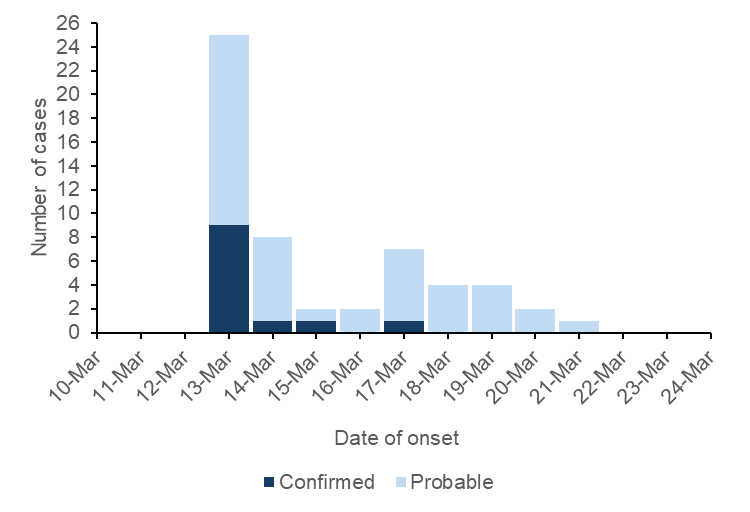
\includegraphics[width=0.95\textwidth]{outbreak/figures/epicurve.png}
%       \caption{Caption goes BELOW the figure.}
%       \label{fig:epicurve}
%   \end{figure}
%   Reference in text: \cref{fig:epicurve}  →  "Figure 1"
%
% HOW TO ADD A TABLE (e.g. attack rate table — save to outbreak/tables/):
%
%   \begin{table}[H]
%       \caption{Caption goes ABOVE the table.}
%       \label{tab:attack_rates}
%       \centering
%       \begin{tabular}{c}
%           \includegraphics[width=0.95\textwidth]{outbreak/tables/attack_rates.png}
%       \end{tabular}
%   \end{table}
%   Reference in text: \cref{tab:attack_rates}  →  "Table 1"

\subsection{Epidemiological investigation}

\subsection{Environmental health investigation}

\subsection{Laboratory investigation}


% =============================================================================
\section{Discussion}
% =============================================================================
Another example of a reference so there's no warnings for this chapter \cite{tasmanian_department_of_health_guidelines_2024}

% =============================================================================
\section{Limitations}
% =============================================================================


% =============================================================================
\section{Conclusion}
% =============================================================================


% =============================================================================
% REFERENCES — do not edit these two lines
% =============================================================================
\clearpage
\addcontentsline{toc}{section}{References}
\printbibliography[heading=subbibliography, title={References}]


% =============================================================================
% APPENDICES
% Uncomment the section(s) relevant to this chapter.
% Upload your files to outbreak/appendices/ before including them.
% REMOVE the entire subappendices block if this chapter has no appendices.
% =============================================================================
\begin{subappendices}

% HOW TO INCLUDE A PDF APPENDIX
% Each page of your PDF is included as a separate \includegraphics line.
% Add or remove \includegraphics lines to match the number of pages in your file.
% Upload your PDF to the outbreak/appendices/ folder before compiling.
% Tip: avoid spaces in filenames — use underscores instead (e.g. my_slides.pdf).

% --- CONFERENCE PRESENTATION SLIDES ---
\clearpage
\section{Conference presentation slides}
\label{app:presentation}
\nopagebreak
\centering

\includegraphics[page=1,width=\textwidth]{outbreak/appendices/Conference presentation slides.pdf}
\clearpage

\includegraphics[page=2,width=\textwidth]{outbreak/appendices/Conference presentation slides.pdf}
% Add more \includegraphics lines here for additional pages
\RaggedRight

% --- MANUSCRIPT ---
\clearpage
\section{Manuscript}
\label{app:manuscript}
\nopagebreak
\centering

\includegraphics[page=1,width=\textwidth]{outbreak/appendices/Manuscript.pdf}
% Add more \includegraphics lines here for additional pages
\RaggedRight

\end{subappendices}
